\chapter{Теоретические основы исследования}

\section{Основные понятия и определения}

Здесь приводятся основные понятия, используемые в работе, их определения и взаимосвязи. В качестве теоретической основы использованы классические работы по программированию \cite{knuth_art} и современные исследования в области машинного обучения \cite{ml_conference}.

\subsection{Понятие 1}

Определение и характеристика первого ключевого понятия.

\begin{figure}[H]
\centering
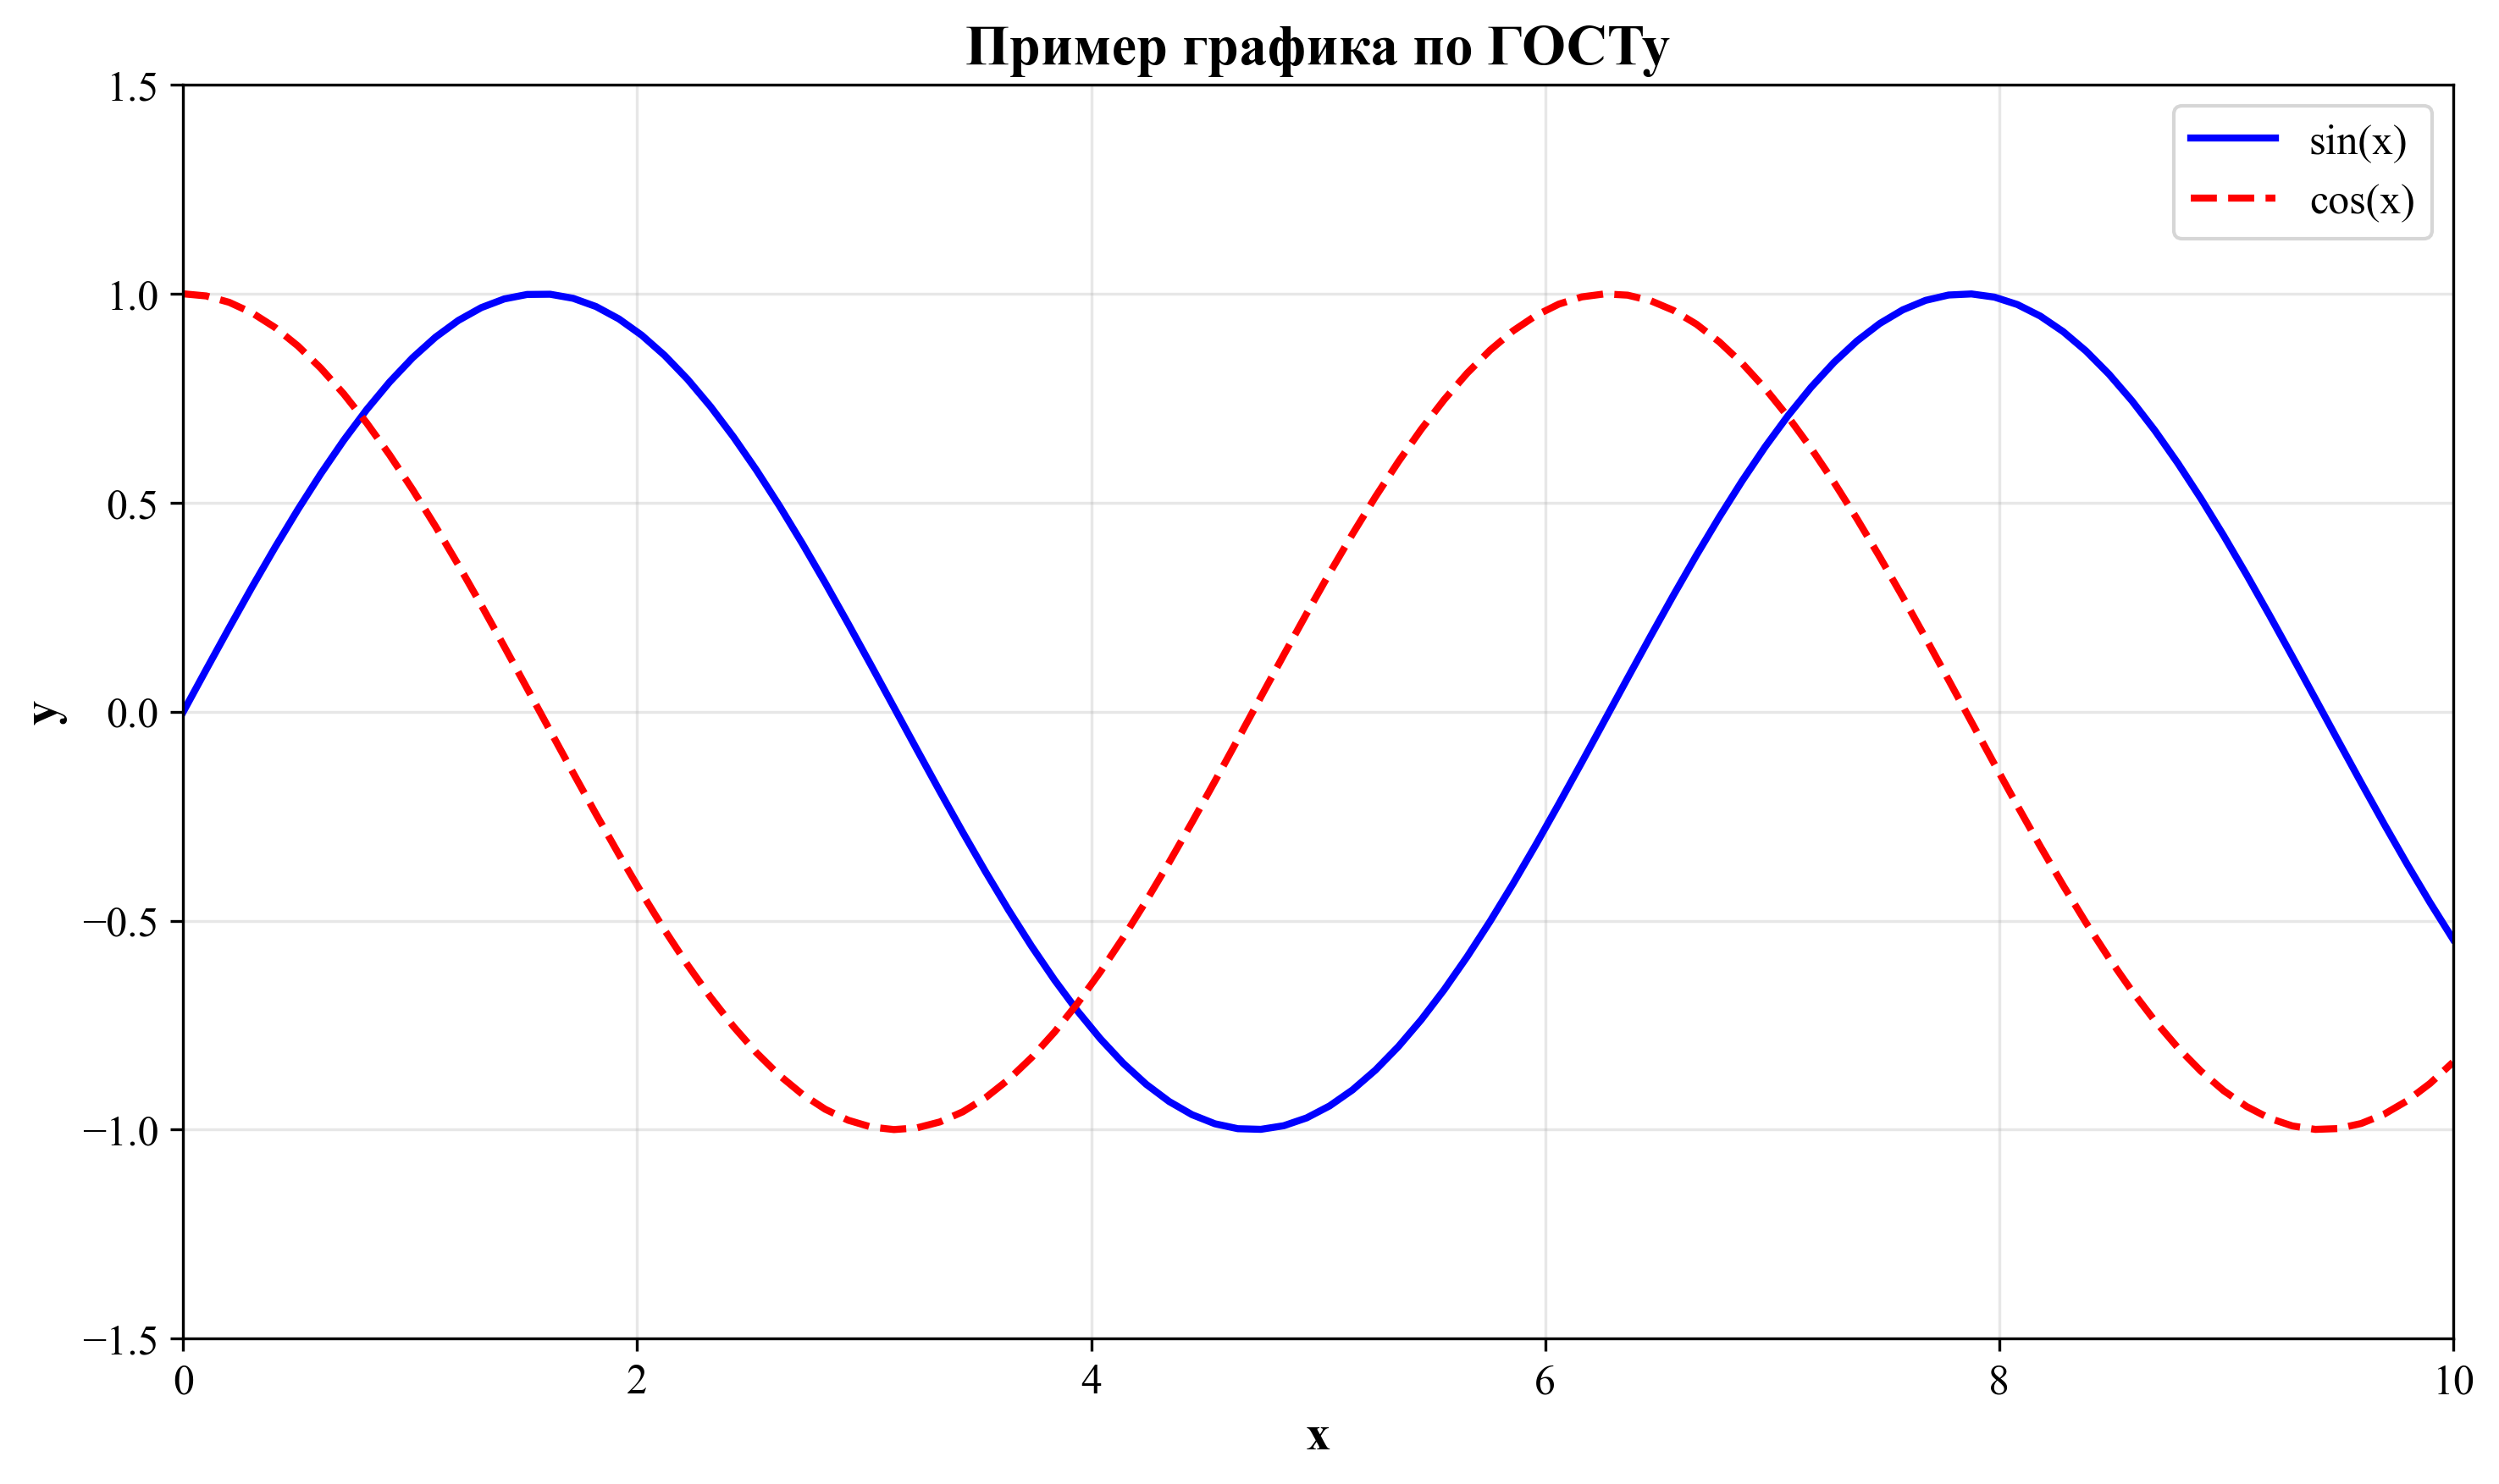
\includegraphics[width=0.8\textwidth]{images/example_plot.png}
\caption{Пример визуализации данных}
\label{fig:data_visualization}
\end{figure}

На рисунке \ref{fig:data_visualization} представлена визуализация исследуемых данных, демонстрирующая основные закономерности.

\begin{table}[H]
\centering
\caption{Основные характеристики данных}
\label{tab:data_characteristics}
\begin{tabular}{|l|c|c|}
\hline
\textbf{Параметр} & \textbf{Значение} & \textbf{Единица измерения} \\
\hline
Количество записей & 1000 & шт. \\
Среднее значение & 15.7 & м/с \\
Стандартное отклонение & 3.2 & м/с \\
\hline
\end{tabular}
\end{table}

В таблице \ref{tab:data_characteristics} приведены основные статистические характеристики исследуемого набора данных.

\begin{equation}
E = mc^2
\label{eq:einstein}
\end{equation}

Формула \ref{eq:einstein} описывает взаимосвязь между массой и энергией.

\begin{lstlisting}[style=code, language=Python, caption={Пример обработки данных}, label={lst:data_processing}]
import pandas as pd
import numpy as np

# Load data
data = pd.read_csv('data.csv')

# Process data
data_clean = data.dropna()
data_processed = data_clean.apply(lambda x: x * 2)

print(f"Processed {len(data_processed)} records")
\end{lstlisting}

В листинге \ref{lst:data_processing} показан пример обработки данных с использованием библиотеки pandas.

\subsection{Понятие 2}

Определение и характеристика второго ключевого понятия.

\section{Анализ существующих подходов}

Обзор и анализ различных подходов к решению исследуемой проблемы.

\subsection{Подход 1}

Описание первого подхода, его достоинства и недостатки.

\subsection{Подход 2}

Описание второго подхода, его достоинства и недостатки.

\section{Методологические основы}

Описание методологических основ исследования.

\section{Выводы по главе}

Краткие выводы по теоретической части работы.
